%%%%%%%%%%%%%%%%%%%%%%%%%%%%%%%%%%%%%%%%%%%%%%%%%%%%%%%%%%%%%%%%%%%%%%%%%%%%%%%
% PREAMBOLO COMUNE PER APPUNTI (Stile Scuro)
%
% Questo file contiene tutte le impostazioni e i pacchetti comuni.
% NON contiene \begin{document} o \end{document}.
%
% Istruzioni per la compilazione del file principale:
% pdflatex -shell-escape nomefile_principale.tex
%%%%%%%%%%%%%%%%%%%%%%%%%%%%%%%%%%%%%%%%%%%%%%%%%%%%%%%%%%%%%%%%%%%%%%%%%%%%%%%

\documentclass{article}

% --- Encoding e lingua ---
\usepackage[utf8]{inputenc}
\usepackage[italian]{babel}

% --- Margini e layout ---
\usepackage{geometry}
\geometry{a4paper, margin=1in}

% --- Font sans-serif (come Helvetica) ---
\usepackage[scaled]{helvet}
\renewcommand{\familydefault}{\sfdefault}
\usepackage[T1]{fontenc}

% --- Matematica ---
\usepackage{amsmath}
\usepackage{amssymb}

% --- Liste personalizzate ---
\usepackage{enumitem}
% \setlist{nosep}

% --- Immagini e Grafica ---
\usepackage{float}
% \usepackage{graphicx}
\usepackage{tikz}
\usetikzlibrary{shapes.geometric, positioning, arrows.meta, calc, fit, backgrounds, patterns, decorations.pathreplacing}

% --- Tabelle Avanzate ---
\usepackage{array}
\usepackage{booktabs}
\usepackage{longtable}

% --- Hyperlink e Metadati PDF ---
\usepackage{hyperref}

\hypersetup{
    colorlinks=true,
    linkcolor=white,
    filecolor=magenta,
    urlcolor=cyan,
    citecolor=green,
    % pdftitle, pdfauthor, ecc. verranno impostati nel file principale
    pdfpagemode=FullScreen,
    bookmarksopen=true,
    bookmarksnumbered=true
}

% --- Licenza del documento ---
\usepackage[
  type={CC},
  modifier={by-sa},
  version={4.0},
]{doclicense}

% --- Colori e Sfondo Nero ---
\usepackage{xcolor}
\pagecolor{black}
\color{white}

% --- Evidenziazione del Codice ---
\usepackage{minted}
\setminted{
    frame=lines,
    framesep=2mm,
    fontsize=\small,
    breaklines=true,
    style=monokai,
    bgcolor=black!80
}
\usemintedstyle{monokai}

% --- Comandi personalizzati per algebra relazionale ---
\newcommand{\Rel}[1]{\textit{#1}} % Per i nomi delle relazioni
\newcommand{\Attr}[1]{\textsf{#1}} % Per i nomi degli attributi

\newcommand{\myunion}{\cup}
\newcommand{\myintersection}{\cap}
\newcommand{\mydifference}{-}
\newcommand{\myrename}[2]{\rho_{#1}(#2)}
\newcommand{\myselectop}[2]{\sigma_{#1}(#2)}
\newcommand{\myproject}[2]{\pi_{#1}(#2)}
\newcommand{\mycartesian}{\times}
\newcommand{\mynaturaljoin}{\bowtie} % Usare \Join da amssymb se disponibile e preferito
\newcommand{\mythetajoin}[3]{#1 \bowtie_{#2} #3} % R1 \bowtie_cond R2

% --- Comandi personalizzati per logica ---
\newcommand{\mylandop}{\wedge}
\newcommand{\myvel}{\vee}
\newcommand{\mynegop}{\neg}
\newcommand{\myforallop}{\forall}
\newcommand{\myexistsop}{\exists}

% --- Join esterni (outer join) ---
% Definizione standard per i join esterni
\def\ojoin{\setbox0=\hbox{$\mynaturaljoin$}%
	\rule[-.02ex]{.25em}{.4pt}\llap{\rule[\ht0]{.25em}{.4pt}}}
\newcommand{\myleftouterjoin}{\mathbin{\ojoin\mkern-5.8mu\mynaturaljoin}}
\newcommand{\myrightouterjoin}{\mathbin{\mynaturaljoin\mkern-5.8mu\ojoin}}
\newcommand{\myfullouterjoin}{\mathbin{\ojoin\mkern-5.8mu\mynaturaljoin\mkern-5.8mu\ojoin}}



% --- Titolo ---
\title{Livello Fisico e Segnali}
\author{Basato sulle slide del Prof. Luciano Bononi}
\date{\today}

\begin{document}

\maketitle
\tableofcontents
\newpage

\section{Background sul Livello Fisico (PHY) Wireless}
Il livello fisico (PHY) si occupa della trasmissione dei bit grezzi attraverso il canale di comunicazione wireless. Comprendere le sue basi è fondamentale per progettare e gestire reti wireless.

\subsection{Proprietà delle Onde Radio (RF - Radio Frequency)}

\subsubsection{Comprensione della Radio Frequenza}
\begin{itemize}
    \item \textbf{Generazione, Copertura e Propagazione:} Le onde RF sono energia elettromagnetica generata da corrente alternata (AC) ad alta frequenza che scorre in un'antenna. L'antenna converte la corrente elettrica ``cablata'' in onde RF e viceversa.
    \item \textbf{Pianificazione Wireless:} La comprensione di come le onde RF si generano e si propagano è cruciale per pianificare la copertura di una rete wireless e gestirla efficacemente.
\end{itemize}
\begin{center}
\begin{tikzpicture}[scale=0.8, every node/.style={transform shape}]
        % Voltaggio
        \begin{scope}[shift={(-2,0)}]
            \draw[->] (0,0) -- (3,0) node[right] {$t$};
            \draw[->] (0,-1) -- (0,1) node[above] {$V$};
            \draw[red, thick] (0,0) sin (0.785,0.8) cos (1.57,-0.8) sin (2.355,0.8) cos (3.14,-0.8);
            \node at (1.5,-1.5) {Voltaggio (AC)};
        \end{scope}
    
        % Antenna (spostata più a destra e migliorata)
        \begin{scope}[shift={(4,0)}]
            % Dipolo verticale (due bracci)
            \draw[thick, themeblue] (4,0.8) -- (4,0.1);  % Braccio superiore
            \draw[thick, themeblue] (4,-0.1) -- (4,-0.8);  % Braccio inferiore
            % Punto di alimentazione (gap e linea di alimentazione)
            \draw[thick, themeblue] (3.7,0) -- (4,0);   % Linea di alimentazione
            \draw[fill=white] (4,0) circle (0.1);  % Punto di alimentazione evidenziato
            \node[right] at (4.3,0) {\small punto di alimentazione};  % Etichetta esplicativa
            \node at (4,-1.5) {Antenna Dipolo};  % Nome più specifico
        
            % Onde RF (migliorate)
            \foreach \i in {1,2,3,4,5} {
                \draw[yellow, opacity=0.9/\i] (4.5+\i*0.25,0) circle (\i*0.5);
            }
            \node at (7,-1.5) {Onde RF};
        \end{scope}
\end{tikzpicture}
\end{center}

\subsubsection{Ampiezza (Amplitude)}
\begin{itemize}
    \item \textbf{Portata:} Segnali RF con ampiezza maggiore (più energia) tendono a propagarsi più lontano.
    \item \textbf{Potenza di Trasmissione (Watts):} È l'energia trasmessa per unità di tempo (Joule/Secondo).
    \[ \text{Potenza } (W) = \text{Tensione } (V) \times \text{Corrente } (A) \]
    Maggiore tensione (energia) muove più elettroni (corrente).
\end{itemize}

\subsubsection{Frequenza (Frequency) e Lunghezza d'Onda (Wavelength)}
\begin{itemize}
    \item \textbf{Spettro Wireless:} L'insieme di tutte le possibili frequenze radio. Solo porzioni di questo spettro sono regolamentate e assegnate a specifiche tecnologie wireless.
    \item \textbf{Relazione:} $\lambda = \frac{c}{f}$
    dove $c$ è la velocità della luce (circa $3 \times 10^8 \, \text{m/s}$) e $f$ è la frequenza in Hertz (Hz).
    \item \textbf{Esempio Pratico (Banda ISM a \SI{2.4}{\giga\hertz}):}
    $f = \SI{2.4}{\giga\hertz} = 2.4 \times 10^9 \, \text{Hz}$
    \[ \lambda = \frac{3 \times 10^8 \, \text{m/s}}{2.4 \times 10^9 \, \text{Hz}} = 0.125 \, \text{m} = \SI{12.5}{\centi\meter} \]
    \item \textbf{Importanza Pratica per le Antenne:} Le antenne funzionano meglio quando la loro dimensione fisica è un multiplo o sottomultiplo della lunghezza d'onda (es. $1, \frac{1}{2}, \frac{1}{4}$ di $\lambda$).
\end{itemize}
\begin{center}
\begin{tikzpicture}[scale=0.9, every node/.style={transform shape}]
    \draw[->] (0,0) -- (5,0) node[right] {Tempo (s)};
    \draw[->] (0,-1.2) -- (0,2.2) node[above] {f};
    % Alta frequenza
    \draw[themeblue, thick] (0.5,1.5) sin (0.75,1.8) cos (1.0,1.2) sin (1.25,1.8) cos (1.5,1.2) sin (1.75,1.8) cos (2.0,1.2) sin (2.25,1.8) cos (2.5,1.2) sin (2.75,1.8) cos (3.0,1.2);
    \node[themeblue] at (1.75,2.2) {Alte Frequenze};
    % Bassa frequenza
    \draw[red, thick] (0.5,0) sin (1.5,0.5) cos (2.5,-0.5) sin (3.5,0.5) cos (4.5,-0.5);
    \node[red] at (2.5,-0.9) {Basse Frequenze};
\end{tikzpicture}
\end{center}

\subsubsection{Fase (Phase)}
\begin{itemize}
    \item \textbf{Definizione:} Sfasamento dell'onda rispetto a un punto di riferimento (gradi o radianti).
    \begin{itemize}
        \item Fase Positiva (left-shift): fronte d'onda anticipato.
        \item Fase Negativa (right-shift): fronte d'onda ritardato.
    \end{itemize}
    \item \textbf{Effetti Pratici (Eco e Interferenza):} Segnali riflessi (echi) arrivano con fasi diverse.
    \begin{itemize}
        \item Se \textbf{in fase}: interferenza costruttiva (segnale più forte).
        \item Se \textbf{in controfase} (sfasate di \SI{180}{\degree}): interferenza distruttiva (segnale più debole o nullo).
    \end{itemize}
\end{itemize}
\begin{center}
    \begin{tikzpicture}[scale=0.9, every node/.style={transform shape}]
        % Axes
        \draw[->] (0,0) -- (7,0) node[right] {Tempo/Fase (gradi)};
        \draw[->] (0,-1.5) -- (0,1.5) node[above] {Ampiezza};
        
        % Reference dashed line
        \draw[dashed, gray] (0,1) -- (6.5,1);
        
        % Signal plots
        % Main signal (phase 0) - themeblue
        \draw[thick, themeblue] plot[domain=0:6.28, samples=100] (\x, {sin(\x r)});
        
        % Phase +90° signal - red
        \draw[thick, red] plot[domain=0:6.28, samples=100] (\x, {sin((\x+1.57) r)*0.5});
        
        % Phase +180° signal - green
        \draw[thick, green] plot[domain=0:6.28, samples=100] (\x, {sin((\x+3.14) r)*0.7});
        
        % Legend in top right corner
        \node[anchor=north east] at (11,2.2) {
            \begin{tabular}{ll}
                \textcolor{themeblue}{---} & Segnale (fase 0) \\
                \textcolor{red}{---} & Segnale (fase +90°) \\
                \textcolor{green}{---} & Segnale (fase +180°)
            \end{tabular}
        };
    \end{tikzpicture}
\end{center}

\subsubsection{Polarizzazione (Polarization)}
\begin{itemize}
    \item \textbf{Definizione:} Orientamento fisico dell'antenna, che determina l'orientamento del campo elettrico dell'onda RF.
    \item \textbf{Componenti Onda RF:} Campo Elettrico (E-field) e Campo Magnetico (H-field), perpendicolari tra loro.
    \item \textbf{Tipi Comuni:}
    \begin{itemize}
        \item Polarizzazione Orizzontale: Campo elettrico parallelo al suolo.
        \item Polarizzazione Verticale: Campo elettrico perpendicolare al suolo (comune nelle WLAN).
    \end{itemize}
    \item \textbf{Importanza Pratica:} Per comunicazione ottimale, le antenne trasmittente e ricevente dovrebbero avere la \textbf{stessa polarizzazione}. Disallineamenti causano perdita di segnale.
\end{itemize}
\begin{center}
\begin{tikzpicture}[scale=0.7, every node/.style={transform shape}]
    % Polarizzazione Verticale
    \node at (-2, 2.5) {Polarizzazione Verticale};
    \draw[thick] (-2,0) -- (-2,2); % Antenna
    \foreach \i in {0.2,0.4,...,1.8} {
        \draw[themeblue, ->] (-2,\i) -- (-1.5,\i); % Campo Elettrico
    }
    \draw[dashed] (-3,-0.5) -- (0,-0.5) node[right] {Suolo};
    % Stickman
    \draw (-2.5, -0.5) -- (-2.5, 0.5) -- (-2.2, 0.2) -- (-2.5, 0.5) -- (-2.8, 0.2);
    \draw (-2.5,0.5) circle (0.2);


    % Polarizzazione Orizzontale
    \node at (3.5, 2.5) {Polarizzazione Orizzontale};
    \draw[thick] (2.5,1) -- (4.5,1); % Antenna
     \foreach \i in {2.7,2.9,...,4.3} {
        \draw[themeblue, ->] (\i,1) -- (\i,1.5); % Campo Elettrico (verso alto per visibilità)
    }
    \draw[dashed] (2,-0.5) -- (5,-0.5) node[right] {Suolo};
    % Stickman
    \draw (3.5, -0.5) -- (3.5, 0.5) -- (3.8, 0.2) -- (3.5, 0.5) -- (3.2, 0.2);
    \draw (3.5,0.5) circle (0.2);
\end{tikzpicture}
\end{center}
\textbf{N.B.:} Il problema della polarizzazione è molto importante per lunghe distanze e antenne direzionali. A breve distanza, le riflessioni mitigano il disallineamento.

\section{Propagazione RF e Comportamenti}

\subsection{Copertura della Trasmissione Radio}
\begin{itemize}
    \item \textbf{Attenuazione con la Distanza:} La potenza del segnale (P) diminuisce con $P \propto \frac{P_{tx}}{d^k}$ (dove $\propto$ significa ``proporzionale a'', $P_{tx}$ è la potenza di trasmissione iniziale e $d^k$ è la distanza elevata all'esponente $k$).
    \begin{itemize}
        \item In spazio libero, $k \approx 2$.
        \item Con ostacoli, $k \ge 3$.
    \end{itemize}
    \item \textbf{Effetto della Potenza di Trasmissione $P_{tx}$:} Aumentando $P_{tx}$, il segnale arriva più lontano.
\end{itemize}

\begin{center}
\begin{tikzpicture}[scale=0.9, every node/.style={transform shape}]
    % Sorgente
    \node[draw, circle, fill=themeblue!30, minimum size=8mm, text=black] (A) at (0,0) {A};
    
    % Onde radio con intensità decrescente
    \draw[themeblue, very thick, opacity=0.9] (A) circle (0.8cm);
    \draw[themeblue, thick, opacity=0.7] (A) circle (1.4cm);
    \draw[themeblue, opacity=0.5] (A) circle (2.0cm);
    \draw[themeblue, opacity=0.3] (A) circle (2.6cm);
    
    % Frecce per indicare la propagazione
    \draw[->, themeblue, thick] (0.6,0.6) -- (1.2,1.2);
    \draw[->, themeblue, thick] (0.6,-0.6) -- (1.2,-1.2);
    \draw[->, themeblue, thick] (-0.6,0.6) -- (-1.2,1.2);
    \draw[->, themeblue, thick] (-0.6,-0.6) -- (-1.2,-1.2);
    
    % Etichette per le zone (più in alto e a destra)
    \node[themeblue, font=\tiny] at (0.85,0.55) {\textbf{Alta}};
    \node[themeblue, font=\tiny] at (1.5,0.75) {\textbf{Media}};
    \node[themeblue, font=\tiny] at (2.07,0.95) {\textbf{Bassa}};
    \node[themeblue, font=\tiny] at (2.9,1.15) {\textbf{Molto bassa}};
    
    % Grafico attenuazione con miglioramenti
    \begin{scope}[xshift=5.5cm, yshift=-3cm]
        \draw[->] (0,0) -- (4.5,0) node[right] {\textbf{Distanza (d)}};
        \draw[->] (0,0) -- (0,6) node[above] {\textbf{Potenza Ricevuta}};
        
        % Curve per diverse potenze di trasmissione (senza etichette)
        \draw[red, very thick] plot[smooth, domain=0.5:4] (\x, {2.8/\x});
        \draw[orange, thick] plot[smooth, domain=0.5:4] (\x, {2.0/\x});
        \draw[themeblue, thick] plot[smooth, domain=0.5:4] (\x, {1.4/\x});
        
        % Legenda in alto a destra
        \node[draw, align=left, font=\small] at (3.5,5) {
            \textcolor{red}{— $P_{tx} = 4W$}\\
            \textcolor{orange}{— $P_{tx} = 2W$}\\
            \textcolor{themeblue}{— $P_{tx} = 1W$}
        };
        
        % Limite di rilevamento
        \draw[primarytext, dashed, thick] (0,0.3) -- (4,0.3) node[right, font=\small] {Limite rilevamento};
        
        % Punti di intersezione per mostrare il range (corretti)
        \fill[red] (3.8,0.3) circle (2pt);
        \fill[orange] (2.6,0.3) circle (2pt);
        \fill[themeblue] (1.8,0.3) circle (2pt);
        
        % Linee verticali per mostrare il range massimo (corrette)
        \draw[red, dotted] (3.8,0) -- (3.8,0.3);
        \draw[orange, dotted] (2.6,0) -- (2.6,0.3);
        \draw[themeblue, dotted] (1.8,0) -- (1.8,0.3);
        
        % Etichette per i range (dentro il grafico)
        \node[red, font=\small] at (3.8,-0.2) {R$_{max}$};
        \node[orange, font=\small] at (2.6,-0.2) {R$_{med}$};
        \node[themeblue, font=\small] at (1.8,-0.2) {R$_{min}$};
    \end{scope}
\end{tikzpicture}
\end{center}

\vspace{0.3cm}
\textbf{Spiegazione dei grafici:}
\begin{itemize}
    \item \textbf{Grafico a sinistra (Propagazione):} Mostra come le onde radio si propagano dalla sorgente A in tutte le direzioni. I cerchi rappresentano zone con diversa intensità del segnale: più ci si allontana dalla sorgente, più il segnale diventa debole.
    
    \item \textbf{Grafico a destra (Attenuazione):} Mostra come la potenza ricevuta diminuisce con la distanza per diverse potenze di trasmissione. Il punto dove ogni curva interseca la linea tratteggiata rappresenta il range massimo di comunicazione per quella potenza.
\end{itemize}

\subsection{Portate (Ranges) della Propagazione del Segnale Wireless}
\begin{itemize}
    \item \textbf{Transmission Range:} Comunicazione possibile con basso tasso di errore.
    \item \textbf{Detection Range:} Segnale rilevabile, ma comunicazione non affidabile.
    \item \textbf{Interference Range:} Segnale abbastanza forte da interferire, anche se non rilevabile.
\end{itemize}
\textbf{Importante:} Queste portate \textbf{dipendono dalla sensibilità del ricevitore!}
\begin{center}
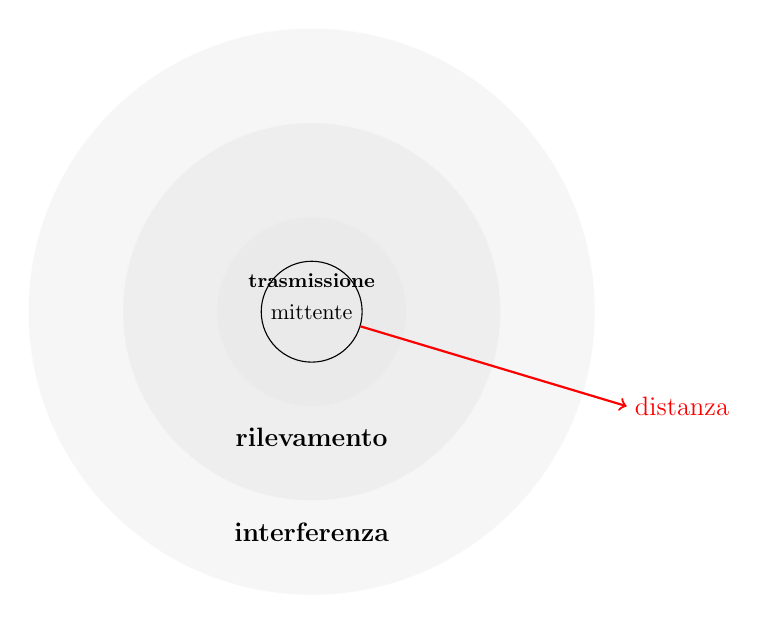
\begin{tikzpicture}[scale=0.8, every node/.style={transform shape}]
    % First draw all the circles with opacity
    \draw[fill=gray!50, draw=white, opacity=0.7] (0,0) circle (1.5cm);
    \draw[fill=gray!30, draw=white, opacity=0.7] (0,0) circle (3cm);
    \draw[fill=gray!10, draw=white, opacity=0.7] (0,0) circle (4.5cm);
    
    % Then add all text nodes without opacity
    \node[draw, circle, text=black] (sender) at (0,0) {mittente};
    \node[text=black, font=\bfseries\small] at (0,0.5cm) {trasmissione};
    \node[text=black, font=\bfseries\large] at (0,-2cm) {rilevamento};
    \node[text=black, font=\bfseries\large] at (0,-3.5cm) {interferenza};
    \draw[->, thick, red] (sender) -- (5, -1.5) node[right, text=red, font=\large] {distanza};
\end{tikzpicture}
\end{center}

\subsection{Effetto degli Ostacoli}
Gli ostacoli possono \textbf{riflettere} o \textbf{assorbire} le onde RF. L'effetto dipende dal materiale e dalla frequenza.
\begin{itemize}
    \item \textbf{Alte Frequenze (es. \SI{5}{\giga\hertz}, \SI{6}{\giga\hertz}):} Più attenuate dagli ostacoli, migliori per brevi distanze.
    \item \textbf{Basse Frequenze (es. \SI{900}{\mega\hertz}):} Penetrano meglio gli ostacoli, migliori per lunghe distanze.
\end{itemize}

\subsection{Effetti della Propagazione del Segnale Wireless}
\begin{itemize}
    \item \textbf{Fading:} Fluttuazioni della potenza del segnale.
    \item \textbf{Shadowing:} Attenuazione da grossi ostacoli.
    \item \textbf{Reflection (Riflessione):} Rimbalzo su grandi superfici.
    \item \textbf{Refraction (Rifrazione):} Cambio direzione attraverso mezzi diversi.
    \item \textbf{Scattering (Diffusione):} Dispersione da piccoli ostacoli.
    \item \textbf{Diffraction (Diffrazione):} Piegamento attorno ai bordi.
\end{itemize}

% Grid layout for propagation effects
\begin{center}
\begin{minipage}[t]{0.48\textwidth}
    \centering
    % 1. REFLECTION (Riflessione)
    \begin{tikzpicture}[scale=0.9]
        \node at (0,3.5) {\textbf{Reflection (Riflessione)}};
        
        % Transmitter
        \fill[red!70] (0,0) circle (0.1);
        \node[below] at (0,-0.2) {TX};
        
        % Receiver
        \fill[blue!70] (4,2) circle (0.1);
        \node[above] at (4,2.2) {RX};
        
        % Edificio/Wall
        \fill[gray!60] (2,-0.5) rectangle (2.5,3);
        \node[rotate=90] at (2.25,1.2) {Edificio};
        
        % Direct path (blocked)
        \draw[red, dashed, thick] (0,0) -- (1.8,1.5);
        \draw[red, thick, cross out, draw=red] (1.9,1.6) circle (0.1);
        
        % Reflected path
        \draw[->, red, thick] (0,0) -- (2,2.5);
        \draw[->, red, thick] (2,2.5) -- (4,2);
        
        % Reflection point
        \fill[green!70] (2,2.5) circle (0.05);
        
        % Angle indicators
        \draw[thin] (1.8,2.5) -- (2.2,2.5);
        \draw[thin] (2,2.3) -- (2,2.7);
        \node[font=\small] at (1.7,2.2) {$\theta_i$};
        \node[font=\small] at (2.3,2.2) {$\theta_r$};
        
        \node[below] at (2,-0.7) {$\theta_i = \theta_r$};
    \end{tikzpicture}
\end{minipage}
\hfill
\begin{minipage}[t]{0.48\textwidth}
    \centering
    % 2. DIFFRACTION (Diffrazione)
    \begin{tikzpicture}[scale=0.9]
        \node at (0,3.5) {\textbf{Diffraction (Diffrazione)}};
        
        % Transmitter
        \fill[red!70] (0,1) circle (0.1);
        \node[below] at (0,0.8) {TX};
        
        % Receiver
        \fill[blue!70] (4,1) circle (0.1);
        \node[below] at (4,0.8) {RX};
        
        % Obstacle (building)
        \fill[gray!60] (1.5,0) rectangle (2.5,2.5);
        \node[rotate=90] at (2,1.2) {Edificio};
        
        % Direct path (blocked)
        \draw[red, dashed, thick] (0,1) -- (1.4,1);
        \draw[red, thick, cross out, draw=red] (1.5,1) circle (0.1);
        
        % Diffracted waves around top edge
        \draw[->, red, thick] (0,1) -- (2,2.5);
        \draw[->, red, thick, bend left=20] (2,2.5) to (4,1);
        
        % Additional diffracted rays
        \draw[->, red!60, thick, bend left=30] (2,2.5) to (3.5,0.5);
        \draw[->, red!60, thick, bend left=10] (2,2.5) to (3.5,1.5);
        
        % Edge point
        \fill[green!70] (2,2.5) circle (0.05);
        \node[right, font=\small] at (2.1,2.5) {Angolo};
        
        % Shadow region
        \fill[black!30, opacity=0.4] (2.5,0) rectangle (4,2);
        \node[font=\small] at (3.2,-0.4) {Shadow Region};
    \end{tikzpicture}
\end{minipage}

\vspace{1cm}

\begin{minipage}[t]{0.48\textwidth}
    \centering
    % 3. SCATTERING (Diffusione)
    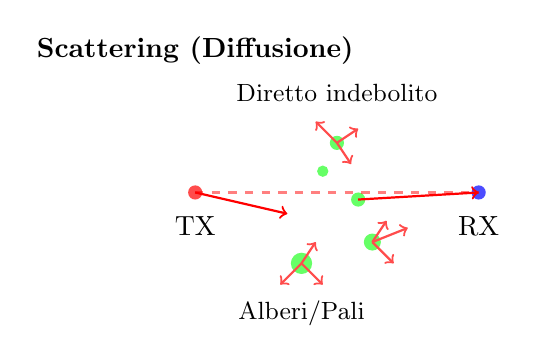
\begin{tikzpicture}[scale=0.9]
        \node at (0,3.5) {\textbf{Scattering (Diffusione)}};
        
        % Transmitter
        \fill[red!70] (0,1.5) circle (0.1);
        \node[below] at (0,1.3) {TX};
        
        % Receiver
        \fill[blue!70] (4,1.5) circle (0.1);
        \node[below] at (4,1.3) {RX};
        
        % Small obstacles (trees, poles, etc.)
        \fill[green!60] (1.5,0.5) circle (0.15);
        \fill[green!60] (2,2.2) circle (0.1);
        \fill[green!60] (2.5,0.8) circle (0.12);
        \fill[green!60] (1.8,1.8) circle (0.08);
        \fill[green!60] (2.3,1.4) circle (0.1);
        
        \node[font=\small] at (1.5,-0.2) {Alberi/Pali};
        
        % Incident wave
        \draw[->, red, thick] (0,1.5) -- (1.3,1.2);
        
        % Scattered waves in multiple directions
        \draw[->, red!70, thick] (1.5,0.5) -- (1.2,0.2);
        \draw[->, red!70, thick] (1.5,0.5) -- (1.8,0.2);
        \draw[->, red!70, thick] (1.5,0.5) -- (1.7,0.8);
        
        \draw[->, red!70, thick] (2,2.2) -- (1.7,2.5);
        \draw[->, red!70, thick] (2,2.2) -- (2.3,2.4);
        \draw[->, red!70, thick] (2,2.2) -- (2.2,1.9);
        
        \draw[->, red!70, thick] (2.5,0.8) -- (2.8,0.5);
        \draw[->, red!70, thick] (2.5,0.8) -- (2.7,1.1);
        \draw[->, red!70, thick] (2.5,0.8) -- (3,1);
        
        % One scattered ray reaching receiver
        \draw[->, red, thick] (2.3,1.4) -- (4,1.5);
        
        % Direct path (weakened)
        \draw[red, dashed, thick, opacity=0.5] (0,1.5) -- (4,1.5);
        \node[font=\small] at (2,2.9) {Diretto indebolito};
    \end{tikzpicture}
\end{minipage}
\hfill
\begin{minipage}[t]{0.48\textwidth}
    \centering
    % 4. MULTIPATH FADING
    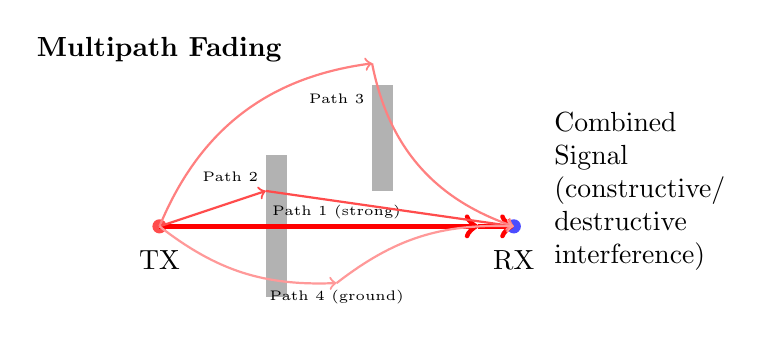
\begin{tikzpicture}[scale=0.9]
        \node at (0,3.5) {\textbf{Multipath Fading}};
        
        % Transmitter
        \fill[red!70] (0,1) circle (0.1);
        \node[below] at (0,0.8) {TX};
        
        % Receiver
        \fill[blue!70] (5,1) circle (0.1);
        \node[below] at (5,0.8) {RX};
        
        % Obstacles
        \fill[gray!60] (1.5,0) rectangle (1.8,2);
        \fill[gray!60] (3,1.5) rectangle (3.3,3);
        
        % Multiple paths with different delays and amplitudes
        % Path 1 - Direct (strongest but partially blocked)
        \draw[->, red, thick, line width=2pt] (0,1) -- (4.5,1);
        \draw[->, red, thick, line width=2pt] (4.5,1) -- (5,1);
        \node[font=\tiny] at (2.5,1.2) {Path 1 (strong)};
        
        % Path 2 - Reflected from building
        \draw[->, red!70, thick] (0,1) -- (1.5,1.5);
        \draw[->, red!70, thick] (1.5,1.5) -- (5,1);
        \node[font=\tiny] at (1,1.7) {Path 2};
        
        % Path 3 - Over building
        \draw[->, red!50, thick, bend left=30] (0,1) to (3,3.3);
        \draw[->, red!50, thick, bend right=30] (3,3.3) to (5,1);
        \node[font=\tiny] at (2.5,2.8) {Path 3};
        
        % Path 4 - Ground reflection
        \draw[->, red!40, thick, bend right=20] (0,1) to (2.5,0.2);
        \draw[->, red!40, thick, bend left=20] (2.5,0.2) to (5,1);
        \node[font=\tiny] at (2.5,0) {Path 4 (ground)};
        
        % Signal combination at receiver
        \node[right] at (5.2,1.5) {\begin{tabular}{l}
            Combined\\
            Signal\\
            (constructive/\\
            destructive\\
            interference)
        \end{tabular}};
    \end{tikzpicture}
\end{minipage}

\vspace{1cm}

\begin{minipage}[t]{0.48\textwidth}
    \centering
    % 5. SHADOWING
    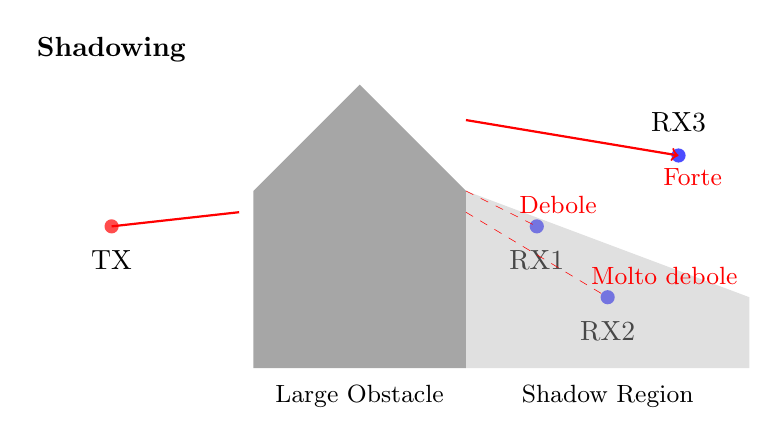
\begin{tikzpicture}[scale=0.9]
        \node at (0,4.5) {\textbf{Shadowing}};
        
        % Transmitter
        \fill[red!70] (0,2) circle (0.1);
        \node[below] at (0,1.8) {TX};
        
        % Large obstacle (mountain/large building)
        \fill[gray!70] (2,0) -- (2,2.5) -- (3.5,4) -- (5,2.5) -- (5,0) -- cycle;
        \node[font=\small] at (3.5,-0.4) {Large Obstacle};
        
        % Receivers at different positions
        \fill[blue!70] (6,2) circle (0.1);
        \node[below] at (6,1.8) {RX1};
        \fill[blue!70] (7,1) circle (0.1);
        \node[below] at (7,0.8) {RX2};
        \fill[blue!70] (8,3) circle (0.1);
        \node[above] at (8,3.2) {RX3};
        
        % Signal strength visualization
        \draw[red, thick] (0,2) -- (1.8,2.2);
        
        % Shadow region
        \fill[black!30, opacity=0.4] (5,0) -- (5,2.5) -- (9,1) -- (9,0) -- cycle;
        \node[font=\small] at (7,-0.4) {Shadow Region};
        
        % Weak signals in shadow
        \draw[red, dashed, very thin] (5,2.5) -- (6,2);
        \draw[red, dashed, very thin] (5,2.2) -- (7,1);
        
        % Strong signal outside shadow
        \draw[->, red, thick] (5,3.5) -- (8,3);
        
        % Signal strength indicators
        \node[font=\small, red] at (6.3,2.3) {Debole};
        \node[font=\small, red] at (7.8,1.3) {Molto debole};
        \node[font=\small, red] at (8.2,2.7) {Forte};
    \end{tikzpicture}
\end{minipage}
\end{center}

\subsection{Propagazione Multipath (Percorsi Multipli)}
Il segnale raggiunge il ricevitore tramite percorsi multipli.
\begin{itemize}
    \item \textbf{Time Dispersion (Dispersione Temporale):} Copie del segnale arrivano in istanti diversi.
    \begin{itemize}
        \item \textbf{Inter-Symbol Interference (ISI):} Sovrapposizione di simboli, causa errori.
    \end{itemize}
    \item \textbf{Distorsione del Segnale:} Il segnale risultante è la somma di copie con fasi e ampiezze diverse.
\end{itemize}

\subsection{Effetti della Mobilità}
Il movimento cambia le caratteristiche del canale.
\begin{itemize}
    \item \textbf{Fading a Breve Termine (Short Term Fading):} Rapide fluttuazioni di potenza.
    \item \textbf{Fading a Lungo Termine (Long Term Fading):} Cambiamenti lenti nella potenza media.
\end{itemize}

\subsection{Voltage Standing Wave Ratio (VSWR)}
\subsubsection{Cos'è il VSWR?}
Il VSWR è un fenomeno che si verifica nei sistemi di trasmissione RF quando c'è un "disadattamento di impedenza" tra i vari componenti.

Con un'analogia, si può immaginare un tubo dell'acqua (il cavo) che collega una pompa (il trasmettitore) a un irrigatore (l'antenna):
\begin{itemize}
    \item Se il tubo ha lo stesso diametro ovunque, l'acqua scorre senza problemi
    \item Se improvvisamente il tubo cambia diametro, parte dell'acqua "rimbalza" indietro, creando turbolenze
\end{itemize}

Allo stesso modo, nelle trasmissioni RF:
\begin{itemize}
    \item L'impedenza (misurata in Ohm $\Omega$) è come il "diametro del tubo" per i segnali RF
    \item Se tutti i componenti hanno la stessa impedenza, il segnale viaggia senza problemi
    \item Se c'è un cambio di impedenza, parte del segnale viene riflesso indietro
\end{itemize}

\subsubsection{Problemi del VSWR}
\begin{itemize}
    \item \textbf{Causa:} Discrepanza di impedenza ($\Omega$) tra trasmettitore, cavo, antenna
    \item \textbf{Effetto (``Return Loss''):} 
    \begin{itemize}
        \item Parte dell'energia viene riflessa indietro verso il trasmettitore
        \item Si creano "onde stazionarie" nel cavo (da qui il nome "Standing Wave")
        \item Meno potenza raggiunge effettivamente l'antenna
    \end{itemize}
    \item \textbf{Conseguenze Negative:} 
    \begin{itemize}
        \item Danneggiamento del trasmettitore (l'energia riflessa può surriscaldarlo)
        \item Instabilità del segnale
        \item Perdita di potenza effettiva trasmessa
        \item Distorsione del segnale
    \end{itemize}
\end{itemize}

\subsubsection{Come si Misura}
\begin{itemize}
    \item Il VSWR è un rapporto tra impedenze, espresso come X:1
    \item VSWR = 1:1 è il caso ideale (nessuna riflessione)
    \item VSWR = 2:1 significa che circa l'11\% della potenza viene riflessa
    \item VSWR = 3:1 significa che circa il 25\% della potenza viene riflessa
\end{itemize}

\subsubsection{Soluzioni}
\begin{itemize}
    \item \textbf{Soluzione Principale:} Usare componenti con la \textbf{stessa impedenza}
    \begin{itemize}
        \item Nelle WLAN moderne si usa tipicamente un'impedenza di \SI{50}{\ohm}
        \item Tutti i componenti (Tx, cavi, antenna) devono essere \SI{50}{\ohm}
    \end{itemize}
    \item \textbf{Alternative:}
    \begin{itemize}
        \item Usare "adattatori di impedenza" tra componenti diversi
        \item Scegliere cavi di alta qualità con impedenza controllata
        \item Minimizzare le giunzioni e i connettori non necessari
    \end{itemize}
\end{itemize}

\begin{center}
    \begin{tikzpicture}[scale=1.2, every node/.style={transform shape}]
        % Trasmettitore
        \node (tx) [draw, rectangle, fill=blue!30, minimum height=1.2cm, minimum width=2.5cm, 
                    text width=2cm, align=center, text=black] at (0,0) {Trasmettitore\\$Z_{out} = \SI{75}{\ohm}$};
        
        % Primo cavo
        \node (cable1) [draw, rectangle, fill=green!30, minimum height=0.8cm, minimum width=2.5cm,
                        text width=2cm, align=center, text=black] at (4,0) {Cavo\\$Z_c = \SI{75}{\ohm}$};
        
        % Secondo cavo
        \node (cable2) [draw, rectangle, fill=red!30, minimum height=0.8cm, minimum width=2.5cm,
                        text width=2cm, align=center, text=black] at (8,0) {Cavo\\$Z_c = \SI{50}{\ohm}$};
        
        % Antenna
        \node (ant) [trapezium, draw, fill=yellow!30, minimum height=1.2cm, minimum width=2cm,
                     shape border rotate=270, text width=1.8cm, align=center, text=black] at (11.5,0) {Antenna\\$Z_L = \SI{50}{\ohm}$};
    
        % Connessioni
        \draw[->, thick] (tx.east) -- (cable1.west);
        \draw[->, thick] (cable1.east) -- (cable2.west);
        \draw[->, thick] (cable2.east) -- (ant.west);
        
        % Etichette VSWR
        \node[above, font=\small\bfseries] at (2, 0.8) {VSWR 1:1};
        \node[above, font=\small\bfseries] at (6, 0.8) {VSWR 1.5:1};
        \node[above, font=\small\bfseries] at (9.75, 0.8) {VSWR 1:1};
        
        % Freccia di riflessione
        \draw[dashed, red, thick, <-] (6, -0.8) to [out=180, in=-30] (5, -1.2);
        \node[below, red, font=\small\bfseries] at (4.5, -1.4) {Riflessione};
        
        % Linee di separazione per chiarezza
        \draw[dotted, gray] (2.75, -1.5) -- (2.75, 1.5);
        \draw[dotted, gray] (6.75, -1.5) -- (6.75, 1.5);
        \draw[dotted, gray] (10.25, -1.5) -- (10.25, 1.5);
        
    \end{tikzpicture}
\end{center}

\section{Potenza e Misurazioni}

\subsection{Radiatore Intenzionale (IR) e EIRP}

\subsubsection{Radiatore Intenzionale (IR)}
\begin{itemize}
    \item È l'insieme di tutti i componenti del sistema di trasmissione \textbf{prima} dell'antenna:
    \begin{itemize}
        \item Trasmettitore RF
        \item Cavi di collegamento
        \item Connettori
    \end{itemize}
    \item La potenza di uscita dell'IR è misurata all'ultimo connettore, immediatamente prima dell'antenna
\end{itemize}

\subsubsection{EIRP (Equivalent Isotropically Radiated Power)}
\begin{itemize}
    \item È una misura teorica che rappresenta la potenza totale del sistema
    \item Definizione: potenza che dovrebbe emettere un'antenna isotropica ideale per produrre la stessa intensità di segnale dell'antenna reale nella direzione di massima emissione
    \item Si calcola come:
    \[ \text{EIRP} (W) = \text{Potenza IR} (W) \times \text{Guadagno Antenna} (\text{rapporto}) \]
    \item In unità logaritmiche (più comunemente usate):
    \[ \text{EIRP} (dBm) = \text{Potenza IR} (dBm) + \text{Guadagno Antenna} (dBi) \]
\end{itemize}

\textbf{Esempi:}
\begin{enumerate}
    \item \textbf{Calcolo in unità lineari:}
    \begin{itemize}
        \item Potenza IR = \SI{0.1}{\watt} = \SI{100}{\milli\watt}
        \item Guadagno antenna = 4 (equivalente a \SI{6}{dBi})
        \item EIRP = \SI{100}{\milli\watt} × 4 = \SI{400}{\milli\watt} = \SI{0.4}{\watt}
    \end{itemize}

    \item \textbf{Calcolo in dB:}
    \begin{itemize}
        \item Potenza IR = \SI{20}{dBm} (\SI{100}{\milli\watt})
        \item Guadagno antenna = \SI{6}{dBi}
        \item EIRP = \SI{20}{dBm} + \SI{6}{dBi} = \SI{26}{dBm} (\SI{400}{\milli\watt})
    \end{itemize}

    \item \textbf{Sistema con perdite:}
    \begin{itemize}
        \item Potenza IR = \SI{30}{dBm} (\SI{1}{\watt})
        \item Perdite nei cavi = \SI{-2}{dB}
        \item Guadagno antenna = \SI{8}{dBi}
        \item EIRP = \SI{30}{dBm} + (\SI{-2}{dB}) + \SI{8}{dBi} = \SI{36}{dBm} (\SI{4}{\watt})
    \end{itemize}
\end{enumerate}

\subsection{Misurazione della Potenza}
\subsubsection{Watt (W) e milliwatt (mW)}
Unità di misura della potenza elettrica \textbf{assoluta}.
\begin{itemize}
    \item Potenza tipica RF per WLAN:
    \begin{itemize}
        \item Access Point (AP): \SIrange{30}{100}{\milli\watt} (fino a \SI{250}{\milli\watt} outdoor).
        \item Client: \SIrange{15}{30}{\milli\watt}.
    \end{itemize}
\end{itemize}

\subsubsection{Decibel (dB)}
Unità logaritmica per esprimere un \textbf{rapporto} tra due potenze (guadagno/perdita).
\[ \text{Guadagno/Perdita (dB)} = 10 \cdot \log_{10} \left( \frac{\text{Potenza}_{\text{uscita}}}{\text{Potenza}_{\text{ingresso}}} \right) \]
\begin{itemize}
    \item Valore dB positivo = guadagno; negativo = perdita.
    \item \textbf{Regole Pratiche Approssimate:}
    \begin{itemize}
        \item $\SI{-3}{dB} \approx 1/2 \text{ potenza}$
        \item $\SI{+3}{dB} \approx 2 \times \text{ potenza}$
        \item $\SI{-10}{dB} \approx 1/10 \text{ potenza}$
        \item $\SI{+10}{dB} \approx 10 \times \text{ potenza}$
    \end{itemize}
    \item \textbf{Vantaggio dei dB:} Guadagni e perdite si sommano algebricamente.
\end{itemize}

\subsubsection{dBm (Decibel-milliWatt)}
Unità logaritmica per misurare la potenza \textbf{assoluta}, con riferimento fisso a \SI{1}{\milli\watt}.
\[ \SI{0}{dBm} = \SI{1}{\milli\watt} \]
\[ \text{Potenza (dBm)} = 10 \cdot \log_{10} \left( \frac{\text{Potenza (mW)}}{\SI{1}{\milli\watt}} \right) \]
\begin{itemize}
    \item Esempi:
    \begin{itemize}
        \item \SI{100}{\milli\watt} = \SI{+20}{dBm}
        \item \SI{30}{\milli\watt} $\approx$ \SI{+14.77}{dBm}
    \end{itemize}
\end{itemize}
\begin{table}[H]
\centering
\begin{tabular}{|c|c|c|c|c|c|c|c|c|c|}
    \hline
    \textbf{dBm} & -30 & -20 & -10 & 0 & +3 & +10 & +20 & +30 & +40 \\ \hline
    \textbf{Potenza} & \SI{1}{\micro\watt} & \SI{10}{\micro\watt} & \SI{0.1}{\milli\watt} & \SI{1}{\milli\watt} & \SI{2}{\milli\watt} & \SI{10}{\milli\watt} & \SI{100}{\milli\watt} & \SI{1}{\watt} & \SI{10}{\watt} \\ \hline
\end{tabular}
\label{tab:dbm_conversion}
\caption{Tabella di Conversione mW -- dBm (approssimata)}
\end{table}

\subsubsection{dBi (Decibel-isotropic)}
Guadagno passivo di un'antenna rispetto a un'antenna \textbf{isotropica} (ideale, 0 dBi gain). Le antenne reali concentrano energia, avendo dBi positivo nelle direzioni preferite.

\subsubsection{dBd (Decibel-dipole)}
Guadagno passivo di un'antenna rispetto a un'antenna \textbf{dipolo a mezz'onda}.
Un dipolo a mezz'onda ha circa $\SI{2.15}{dBi}$.
\[ \SI{0}{dBd} = \SI{2.15}{dBi} \]
\[ \text{Guadagno (dBi)} = \text{Guadagno (dBd)} + 2.15 \]

\subsection{Monitoraggio della Potenza (es. IEEE 802.11)}
\begin{itemize}
    \item \textbf{Necessità:} Per determinare soglia sensibilità, selezionare bitrate, verificare stato canale.
    \item \textbf{RSSI (Received Signal Strength Indicator):} Indice della potenza ricevuta.
    \item \textbf{Problema:} Scala RSSI \textbf{non standardizzata} tra produttori. Difficile confrontare dispositivi basandosi solo su RSSI grezzo. Meglio guardare al valore in dBm.
\end{itemize}

\section{Antenne}

\subsection{Questioni Generali}
\begin{itemize}
    \item \textbf{Funzione:} Convertono energia elettrica $\leftrightarrow$ onde RF.
    \item \textbf{Dimensione:} Correlata alla frequenza RF (lunghezza d'onda).
    \item \textbf{Forma:} Correlata al pattern di radiazione.
    \item \textbf{Posizionamento:} Cruciale per copertura e sicurezza.
\end{itemize}

\subsection{Antenna Omnidirezionale (es. Dipolo)}
Irradia potenza equamente attorno all'asse verticale (pattern a ``ciambella'').
\begin{itemize}
    \item \textbf{Dipolo a basso guadagno (es. \SI{2}{dBi}):} Ciambella più ``grassa'', buona copertura verticale.
    \item \textbf{Dipolo ad alto guadagno (es. \SIrange{8}{10}{dBi}):} Ciambella ``piatta'' e larga, buona copertura orizzontale estesa.
    \item \textbf{N.B.:} Segnale debole sopra/sotto un dipolo verticale (nel ``buco della ciambella'').
    \item \textbf{Tilt dell'Antenna (Inclinazione):} Inclinare un'antenna ad alto guadagno verso il basso (``downtilt'') migliora la copertura nell'area sottostante.
\end{itemize}
\begin{center}
\begin{tikzpicture}[scale=0.8, every node/.style={transform shape}]
    % Vista Laterale (Side View)
    \node[font=\bfseries] at (-4,4) {Vista Laterale};
    
    % Low Gain Dipole - Side View
    \begin{scope}[shift={(-6,0)}]
        \node[font=\bfseries] at (0,3) {Dipolo Basso Guadagno};
        % Antenna
        \draw[thick, themeblue] (0,-0.5) -- (0,2);
        % Pattern di radiazione
        \fill[red!20, opacity=0.3] (0,0.75) ellipse (2cm and 1.5cm);
        \draw[red, thick] (0,0.75) ellipse (2cm and 1.5cm);
        % Linee di campo
        \foreach \angle in {0,30,...,330} {
            \draw[->, red!70, thin] (0,0.75) -- ++ (\angle:1cm);
        }
        % Label
        \node[text width=2cm, align=center, font=\small] at (0,-1.8) {2 dBi\\Copertura verticale migliore};
    \end{scope}
    
    % High Gain Dipole - Side View
    \begin{scope}[shift={(0,0)}]
        \node[font=\bfseries] at (0,3) {Dipolo Alto Guadagno};
        % Antenna
        \draw[thick, themeblue] (0,-0.5) -- (0,2);
        % Pattern di radiazione
        \fill[themeblue!20, opacity=0.3] (0,0.75) ellipse (3cm and 0.8cm);
        \draw[themeblue, thick] (0,0.75) ellipse (3cm and 0.8cm);
        % Linee di campo
        \foreach \angle in {0,30,...,330} {
            \draw[->, themeblue!70, thin] (0,0.75) -- ++ (\angle:1.5cm);
        }
        % Label
        \node[text width=2cm, align=center, font=\small] at (0,-1.8) {8-10 dBi\\Copertura orizzontale migliore};
    \end{scope}

    % Vista dall'Alto (Top View)
    \node[font=\bfseries] at (-4,-3.5) {Vista dall'Alto};
    
    % Low Gain Dipole - Top View
    \begin{scope}[shift={(-6,-6)}]
        % Antenna (punto centrale)
        \fill[themeblue] (0,0) circle (0.1);
        % Pattern di radiazione circolare
        \fill[red!20, opacity=0.3] (0,0) circle (2cm);
        \draw[red, thick] (0,0) circle (2cm);
        % Linee di campo radiali
        \foreach \angle in {0,45,...,315} {
            \draw[->, red!70, thin] (0,0) -- ++ (\angle:1.5cm);
        }
        % Label
        \node[font=\small] at (0,-2.5) {Pattern circolare uniforme};
    \end{scope}
    
    % High Gain Dipole - Top View
    \begin{scope}[shift={(0,-6)}]
        % Antenna (punto centrale)
        \fill[themeblue] (0,0) circle (0.1);
        % Pattern di radiazione circolare ma più ampio
        \fill[themeblue!20, opacity=0.3] (0,0) circle (3cm);
        \draw[themeblue, thick] (0,0) circle (3cm);
        % Linee di campo radiali più lunghe
        \foreach \angle in {0,45,...,315} {
            \draw[->, themeblue!70, thin] (0,0) -- ++ (\angle:2.5cm);
        }
        % Label
        \node[font=\small] at (0,-3.5) {Copertura più estesa};
    \end{scope}

    % Legenda
    \begin{scope}[shift={(4,-3)}]
        \node[draw, align=left, font=\small] {
            \textcolor{red}{— Basso guadagno (2 dBi)}\\
            \textcolor{themeblue}{— Alto guadagno (8-10 dBi)}\\
            \textcolor{themeblue}{• Antenna}
        };
    \end{scope}
\end{tikzpicture}
\end{center}

\subsection{Antenne Semi-Direzionali}
Concentrano energia in una direzione più specifica.
\begin{itemize}
    \item \textbf{Tipi:} Patch, Panel (piatte, a muro), Yagi (asta con ``baffi'').
    \item \textbf{Beamwidth (Larghezza del Fascio):} Angolo entro cui la potenza è almeno -3dB rispetto al massimo.
\end{itemize}

\subsection{Antenne Altamente-Direzionali}
Concentrano energia in un fascio molto stretto, alto guadagno.
\begin{itemize}
    \item \textbf{Tipi:} Parabolic Dish, Grid.
    \item \textbf{Uso Comune:} Link Punto-Punto (LOS).
    \item \textbf{Allineamento Critico.}
    \item \textbf{Fresnel Zone (Zona di Fresnel):} Spazio a forma di ellissoide attorno al LOS. La prima FZ deve essere il più libera possibile da ostruzioni.
    \begin{itemize}
        \item Raggio FZ dipende da distanza e frequenza, \textbf{non} dal tipo di antenna.
        \item Ostruzione < 20\% tollerabile.
        \item \textbf{Curvatura Terrestre:} Importante per link > \SI{10}{\kilo\meter}.
    \end{itemize}
\end{itemize}
\begin{center}
    \begin{tikzpicture}[scale=1.2, every node/.style={transform shape}]
        % Define antenna style
        \tikzset{
            antenna/.style={
                cylinder, 
                draw=blue!80!black, 
                thick,
                shape border rotate=90, 
                aspect=0.4, 
                minimum height=1.5cm, 
                minimum width=0.7cm, 
                fill=blue!20
            }
        }
    
        % Antenna positions
        \coordinate (tx_pos) at (-4.5,0.75);
        \coordinate (rx_pos) at (4.5,0.75);
    
        % Antenna bases
        \fill[gray!40] (-5,-0.5) rectangle (-4,0);
        \fill[gray!40] (4,-0.5) rectangle (5,0);
        
        % Antennas
        \node (tx_ant) at (tx_pos) [antenna] {};
        \node (rx_ant) at (rx_pos) [antenna] {};
        
        % Antenna labels
        \node[below, font=\small] at (-4.5,-0.7) {Antenna TX};
        \node[below, font=\small] at (4.5,-0.7) {Antenna RX};
    
        % Fresnel Zone ellipse (drawn first, behind other elements)
        \draw[orange, thick] (0,0.75) ellipse (4.2cm and 1.1cm);
        \fill[orange!15, opacity=0.4] (0,0.75) ellipse (4.2cm and 1.1cm);
    
        % Line of Sight
        \draw[dashed, red, thick] (tx_ant.east) -- (rx_ant.west);
        
        % LOS label positioned above the Fresnel zone
        \node[above, font=\small, text=red] at (0,2.1) {Line of Sight (LOS)};
    
        % Fresnel zone label positioned below the center line
        \node[font=\small, text=orange!80!black] at (0,-0.1) {Prima Zona di Fresnel};
    
        % Obstacles
        % Large obstacle on the left
        \fill[green!50] (-2,0.2) circle (0.4cm);
        \node[below, font=\footnotesize] at (-2,-0.4) {Ostacolo};
        
        % Smaller obstacle on the right
        \fill[green!40] (1.2,0.5) circle (0.25cm);
    
        % Fresnel radius indicator
        \draw[<->, black, thin] (0,0.75) -- (0,1.85) 
            node[midway, text=black, right, font=\footnotesize] {Raggio Fresnel};
    
        % Legend positioned to avoid overlap
        \node[draw, fill=white, text=black, align=left, font=\footnotesize, 
              drop shadow, rounded corners=2pt] at (6.5,1.5) {
            \textcolor{red}{\rule{0.8cm}{0.8pt}} Line of Sight\\[2pt]
            \textcolor{orange}{\rule{0.8cm}{0.8pt}} Zona di Fresnel\\[2pt]
            \textcolor{green!60!black}{$\bullet$} Ostacoli\\[2pt]
            \textcolor{blue!80!black}{$\blacksquare$} Antenne
        };
    
    \end{tikzpicture}
\end{center}

\subsection{Antenne Settorizzate-Direzionali}
Array di antenne direzionali per coprire settori specifici. Permettono Space Multiplexing (riuso canali).

\subsection{Grafici di Copertura Antenna (Azimuth e Elevation)}
Diagrammi polari della potenza relativa nelle varie direzioni.
\begin{itemize}
    \item \textbf{Azimuth Chart:} Pattern visto dall'alto.
    \item \textbf{Elevation Chart:} Pattern visto di lato.
\end{itemize}

\subsection{Diversità delle Antenne (Antenna Diversity)}
Uso di più antenne per combattere il multipath fading.
\begin{itemize}
    \item \textbf{Switched/Selection Diversity:} Il ricevitore sceglie l'antenna con segnale migliore.
    \item \textbf{Diversity Combining:} I segnali vengono combinati (può richiedere cophasing).
\end{itemize}

\section{Path Loss e Link Budget}

\subsection{Path Loss (Perdita di Percorso)}
Attenuazione del segnale con distanza e frequenza.
\begin{itemize}
    \item Formula Free Space Path Loss (FSPL) (esempio):
    \[ \text{FSPL (dB)} = 32.4 + 20 \log_{10}(f_{MHz}) + 20 \log_{10}(d_{km}) \]
    \item \textbf{Regola dei 6 dB:} Ogni $\SI{+6}{dB}$ in EIRP (potenza x4) circa raddoppia la portata Tx (assumendo attenuazione $d^2$).
\end{itemize}
\begin{table}[H]
\centering
\caption{Esempio Path Loss 2.4 GHz vs Distanza (valori indicativi)}
\begin{tabular}{|c|c|c|}
\hline
\textbf{Distanza} & \textbf{Path Loss (dB)} & \textbf{Variazione approx.} \\ \hline
\SI{100}{\meter} & \SI{-80.2}{dB} & - \\ \hline
\SI{200}{\meter} & \SI{-86.2}{dB} & $\approx \SI{-6}{dB}$ \\ \hline
\SI{500}{\meter} & \SI{-94.2}{dB} & $\approx \SI{-8}{dB}$ \\ \hline
\SI{1000}{\meter} & \SI{-100.2}{dB} & $\approx \SI{-6}{dB}$ \\ \hline
\end{tabular}
\label{tab:path_loss}
\end{table}

\subsection{Calcolo del Link Budget (System Operating Margin)}
Eccesso di segnale rispetto al minimo necessario.
\begin{itemize}
    \item \textbf{Sensibilità del Ricevitore (RS):} Potenza minima (dBm) per decodifica affidabile. Più basso è, meglio è. Dipende dal bitrate.
    \item \textbf{Calcolo Potenza Ricevuta ($P_{RX}$):}
    \[ P_{RX} (\text{dBm}) = P_{TX} (\text{dBm}) + G_{TX} (\text{dBi}) + G_{RX} (\text{dBi}) - L_{\text{cavi}} (\text{dB}) - \text{PathLoss} (\text{dB}) \]
    \item \textbf{Link Budget (dB):}
    \[ \text{Link Budget} = P_{RX} (\text{dBm}) - RS (\text{dBm}) \]
    \item \textbf{Fade Margin (Margine di Fading):} Margine extra (tipico $\SIrange{+10}{+20}{dB}$) per fluttuazioni.
    \[ P_{RX} (\text{dBm}) > RS (\text{dBm}) + \text{Fade Margin (dB)} \]
\end{itemize}
\textbf{Esempio Link Budget (dalla slide 58, valori semplificati concettualmente):}
\begin{itemize}
    \item $P_{TX} = \SI{+15}{dBm}$
    \item $G_{TX} = \SI{+24}{dBi}$, $G_{RX} = \SI{+24}{dBi}$
    \item $L_{\text{cavi totali}} = \SI{10.8}{dB}$
    \item Path Loss (\SI{10}{km}) = $\SI{120}{dB}$
    \item $RS = \SI{-82}{dBm}$
    \item $P_{RX} = \SI{15}{dBm} + \SI{24}{dBi} + \SI{24}{dBi} - \SI{10.8}{dB} - \SI{120}{dB} = \SI{-67.8}{dBm}$
    \item Link Budget = $\SI{-67.8}{dBm} - (\SI{-82}{dBm}) = \SI{+14.2}{dB}$
\end{itemize}
Questo margine di $\SI{14.2}{dB}$ è disponibile per il fading. Se il fade margin richiesto è, ad esempio, $\SI{10}{dB}$, il link è considerato affidabile.

\section{Approfondimento: Path Loss e Link Budget nella Pratica}

\subsection{Path Loss in Dettaglio}
Il Path Loss è fondamentale per capire come si attenua il segnale wireless. Vediamo alcuni esempi pratici:

\begin{center}
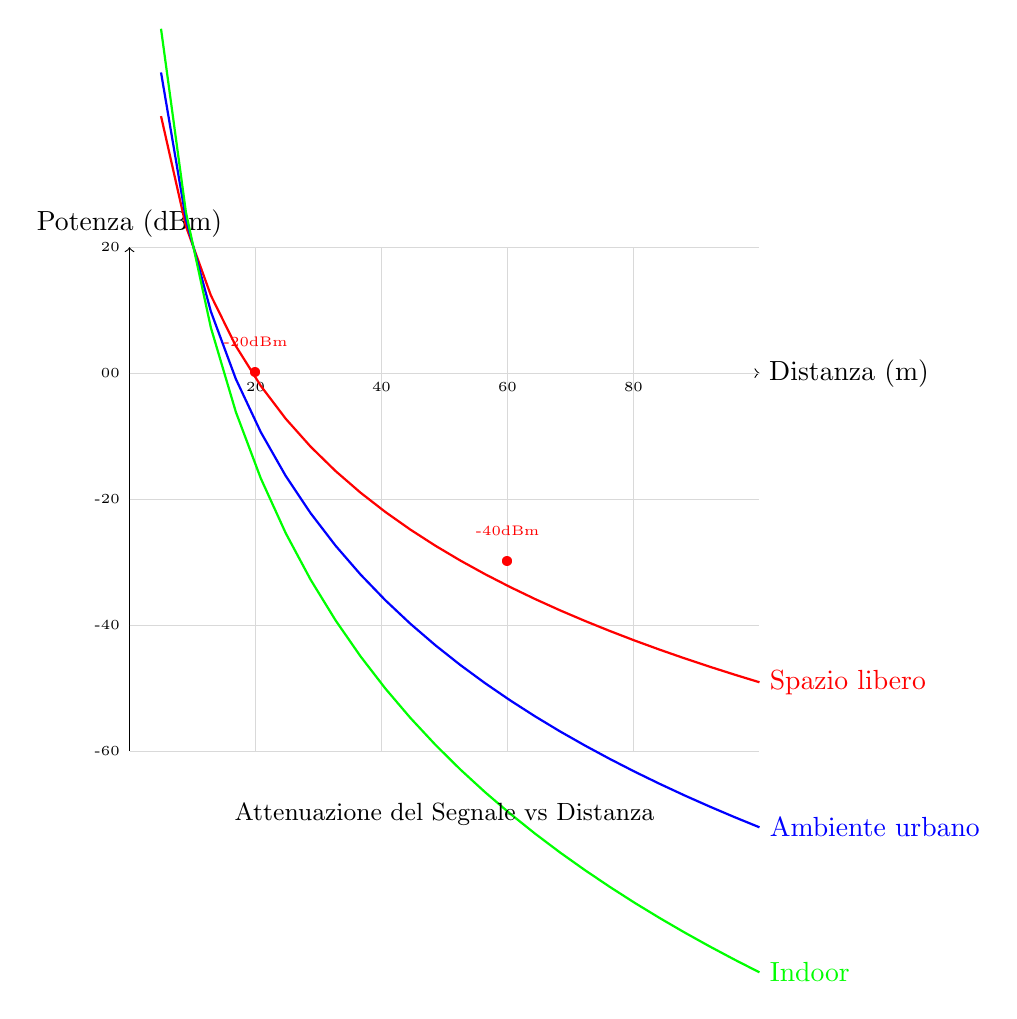
\begin{tikzpicture}[scale=0.8]
    % Asse X (distanza)
    \draw[->] (0,0) -- (10,0) node[right] {Distanza (m)};
    \draw[->] (0,-6) -- (0,2) node[above] {Potenza (dBm)};
    
    % Griglia di riferimento
    \foreach \y in {-6,-4,-2,0,2} {
        \draw[gray!30] (0,\y) -- (10,\y);
        \node[left, font=\tiny] at (0,\y) {\y0};
    }
    \foreach \x in {2,4,6,8} {
        \draw[gray!30] (\x,-6) -- (\x,2);
        \node[below, font=\tiny] at (\x,0) {\x0};
    }
    
    % Curve di attenuazione
    \draw[red, thick] plot[domain=0.5:10] (\x,{2-3*ln(\x)}) 
        node[right] {Spazio libero};
    \draw[blue, thick] plot[domain=0.5:10] (\x,{2-4*ln(\x)}) 
        node[right] {Ambiente urbano};
    \draw[green, thick] plot[domain=0.5:10] (\x,{2-5*ln(\x)}) 
        node[right] {Indoor};
    
    % Punti di riferimento
    \node[red, font=\small] at (2,0) {•};
    \node[red, font=\tiny] at (2,0.5) {-20dBm};
    \node[red, font=\small] at (6,-3) {•};
    \node[red, font=\tiny] at (6,-2.5) {-40dBm};
    
    \node[font=\small] at (5,-7) {Attenuazione del Segnale vs Distanza};
\end{tikzpicture}
\end{center}

\subsubsection{Esempi Pratici di Path Loss}
\begin{itemize}
    \item \textbf{Scenario Indoor (Ufficio):}
    \begin{itemize}
        \item Access Point WiFi: \SI{20}{dBm} (\SI{100}{mW})
        \item Distanza client: \SI{10}{m}
        \item Ostacoli: 2 pareti (\SI{-4}{dB} ciascuna)
        \item Path Loss calcolato: \SI{-40}{dB} + (\SI{-8}{dB}) = \SI{-48}{dB}
        \item Potenza ricevuta: \SI{20}{dBm} - \SI{48}{dB} = \SI{-28}{dBm}
    \end{itemize}
    
    \item \textbf{Scenario Outdoor (Parco):}
    \begin{itemize}
        \item Access Point: \SI{30}{dBm} (\SI{1}{W})
        \item Distanza client: \SI{100}{m}
        \item Path Loss calcolato: \SI{-80}{dB}
        \item Potenza ricevuta: \SI{30}{dBm} - \SI{80}{dB} = \SI{-50}{dBm}
    \end{itemize}
\end{itemize}

\subsection{Link Budget Visualizzato}
Il Link Budget è come un "bilancio energetico" del sistema wireless:

\begin{center}
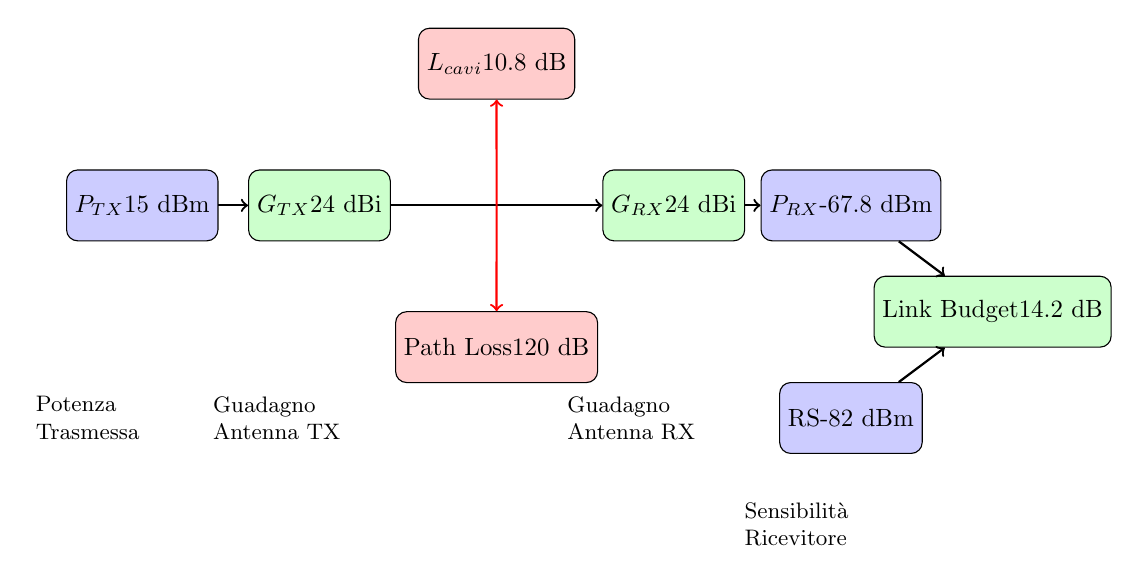
\begin{tikzpicture}[scale=0.9, every node/.style={transform shape}]
    % Definizione stili
    \tikzset{
        block/.style={rectangle, draw, fill=blue!20, 
                     minimum height=1cm, minimum width=2cm,
                     text centered, rounded corners},
        loss/.style={rectangle, draw, fill=red!20,
                    minimum height=1cm, minimum width=2cm,
                    text centered, rounded corners},
        gain/.style={rectangle, draw, fill=green!20,
                    minimum height=1cm, minimum width=2cm,
                    text centered, rounded corners}
    }
    
    % Trasmettitore
    \node[block, text=black] (tx) at (0,0) {$P_{TX}$\\15 dBm};
    
    % Guadagni antenne
    \node[gain, text=black] (gtx) at (2.5,0) {$G_{TX}$\\24 dBi};
    \node[gain, text=black] (grx) at (7.5,0) {$G_{RX}$\\24 dBi};
    
    % Perdite
    \node[loss, text=black] (lcavi) at (5,2) {$L_{cavi}$\\10.8 dB};
    \node[loss, text=black] (lpath) at (5,-2) {Path Loss\\120 dB};
    
    % Ricevitore
    \node[block, text=black] (rx) at (10,0) {$P_{RX}$\\-67.8 dBm};
    
    % Sensibilità
    \node[block, text=black] (rs) at (10,-3) {RS\\-82 dBm};
    
    % Link Budget
    \node[gain, text=black] (lb) at (12,-1.5) {Link Budget\\14.2 dB};
    
    % Connessioni
    \draw[->, thick] (tx) -- (gtx);
    \draw[->, thick] (gtx) -- (grx);
    \draw[->, thick] (grx) -- (rx);
    \draw[->, thick, red] (5,0) -- (lcavi);
    \draw[->, thick, red] (5,0) -- (lpath);
    \draw[->, thick] (rx) -- (lb);
    \draw[->, thick] (rs) -- (lb);
    
    % Spiegazioni
    \node[text width=3cm, align=left, font=\small] at (0,-3) 
        {Potenza\\Trasmessa};
    \node[text width=3cm, align=left, font=\small] at (2.5,-3) 
        {Guadagno\\Antenna TX};
    \node[text width=3cm, align=left, font=\small] at (7.5,-3) 
        {Guadagno\\Antenna RX};
    \node[text width=3cm, align=left, font=\small] at (10,-4.5) 
        {Sensibilità\\Ricevitore};
\end{tikzpicture}
\end{center}

\subsection{Scenari di Link Budget}
\begin{table}[H]
\centering
\caption{Comparazione Scenari Link Budget}
\begin{tabular}{|l|c|c|c|}
\hline
\textbf{Parametro} & \textbf{Indoor} & \textbf{Outdoor} & \textbf{Long Range} \\
\hline
$P_{TX}$ & \SI{15}{dBm} & \SI{20}{dBm} & \SI{30}{dBm} \\
$G_{TX}$ & \SI{3}{dBi} & \SI{6}{dBi} & \SI{24}{dBi} \\
$G_{RX}$ & \SI{2}{dBi} & \SI{6}{dBi} & \SI{24}{dBi} \\
$L_{cavi}$ & \SI{2}{dB} & \SI{4}{dB} & \SI{10}{dB} \\
Path Loss & \SI{60}{dB} & \SI{90}{dB} & \SI{120}{dB} \\
$P_{RX}$ & \SI{-42}{dBm} & \SI{-62}{dBm} & \SI{-52}{dBm} \\
RS & \SI{-70}{dBm} & \SI{-75}{dBm} & \SI{-82}{dBm} \\
\hline
Link Budget & \SI{28}{dB} & \SI{13}{dB} & \SI{30}{dB} \\
\hline
\end{tabular}
\end{table}

\textbf{Esempi di Applicazione:}
\begin{itemize}
    \item \textbf{Indoor:} WiFi domestico, copertura appartamento
    \begin{itemize}
        \item Distanze brevi (\SI{5}-\SI{20}{m})
        \item Antenne omnidirezionali a basso guadagno
        \item Ostacoli: muri, mobili
    \end{itemize}
    
    \item \textbf{Outdoor:} WiFi pubblico, parchi
    \begin{itemize}
        \item Distanze medie (\SI{50}-\SI{200}{m})
        \item Antenne settoriali
        \item Pochi ostacoli
    \end{itemize}
    
    \item \textbf{Long Range:} Ponte radio punto-punto
    \begin{itemize}
        \item Lunghe distanze (\SI{1}-\SI{10}{km})
        \item Antenne direttive ad alto guadagno
        \item Line of Sight necessaria
    \end{itemize}
\end{itemize}

\begin{center}
\begin{tikzpicture}[scale=0.7]
    % Definizione degli scenari
    \begin{scope}[shift={(-6,-0.6)}]  % Added -1 to y-shift
        \node[font=\bfseries] at (0,3.5) {Indoor};
        % Casa
        \draw[thick] (-2,0) rectangle (2,2);
        \draw (-2,2) -- (0,3) -- (2,2); % tetto
        % AP e client
        \fill[red] (-1,1) circle (0.1) node[below] {AP};
        \fill[themeblue] (1,1) circle (0.1) node[below] {Client};
        % Segnale
        \draw[red,thick,decorate,decoration={snake,amplitude=0.3mm}] 
            (-1,1) -- (1,1);
    \end{scope}
    
    \begin{scope}[shift={(0,0)}]
        \node[font=\bfseries] at (0,3) {Outdoor};
        % Area
        \draw[thick] (-2.5,-0.5) rectangle (2.5,2);
        % AP e clients
        \fill[red] (0,2) circle (0.1) node[above] {AP};
        \fill[themeblue] (-2,0) circle (0.1) node[below] {C1};
        \fill[themeblue] (0,0) circle (0.1) node[below] {C2};
        \fill[themeblue] (2,0) circle (0.1) node[below] {C3};
        % Segnali
        \foreach \x in {-2,0,2} {
            \draw[red,thick,decorate,decoration={snake,amplitude=0.3mm}] 
                (0,2) -- (\x,0);
        }
    \end{scope}
    
    \begin{scope}[shift={(6,0)}]
        \node[font=\bfseries] at (0,3) {Long Range};
        % Torri
        \draw[thick] (-2,0) rectangle (-1.5,2);
        \draw[thick] (1.5,0) rectangle (2,2);
        % Antenne
        \draw[thick] (-1.5,1.8) -- (-1,1.8) -- (-1,1.2) -- (-1.5,1.2);
        \draw[thick] (1.5,1.8) -- (2,1.8) -- (2,1.2) -- (1.5,1.2);
        % Segnale direttivo
        \draw[red,thick,decorate,decoration={snake,amplitude=0.4mm}] 
            (-1,1.5) -- (1.5,1.5);
        % Distanza
        \draw[<->] (-2,-0.5) -- (2,-0.5) 
            node[midway,below] {\SI{1}-\SI{10}{km}};
    \end{scope}
\end{tikzpicture}
\end{center}

\end{document}